\section{KẾT QUẢ THỰC NGHIỆM VÀ THẢO LUẬN}

\subsection{Kết quả đánh giá cuối}

Sau 20.000 episode training, cả chín cấu hình được evaluation độc lập trên 20 episode với $\epsilon=0$. Tất cả cấu hình sử dụng training seed 42 và evaluation seed 10042. Hai seed được tách riêng, còn evaluation seed được giữ cố định nhằm tăng tính nhất quán và khả năng tái lập kết quả. \tabref{tab:final-eval-results} tổng hợp kết quả của lần evaluation cuối tại episode 20.000 \cite{DRLPacmanGitHub}.

\begin{table}[H]
    \centering
    \renewcommand{\arraystretch}{1.2}
    \small
    \begin{tabularx}{\textwidth}{@{}
        >{\raggedright\arraybackslash}p{2.4cm}
        >{\centering\arraybackslash}p{1.1cm}
        >{\centering\arraybackslash}p{1.9cm}
        >{\centering\arraybackslash}p{2.6cm}
        >{\centering\arraybackslash}p{1.4cm}
        >{\centering\arraybackslash}p{1.5cm}
        >{\centering\arraybackslash}X
    @{}}
        \toprule
        \textbf{Thuật toán} & \textbf{LR} & \textbf{Reward Avg} & \textbf{Completion Avg} & \textbf{Win Rate} & \textbf{Steps Avg} & \textbf{Completion Max} \\
        \midrule
        Double DQN & $0{,}0001$ & $1247{,}154$ & $99{,}76\%$ & $95\%$ & $148{,}30$ & $100\%$ \\
        Double DQN & $0{,}0005$ & $1312{,}231$ & $99{,}27\%$ & $85\%$ & $153{,}60$ & $100\%$ \\
        Double DQN & $0{,}001$ & $1553{,}422$ & $99{,}27\%$ & $65\%$ & $211{,}65$ & $100\%$ \\
        DQN & $0{,}0001$ & $1125{,}694$ & $98{,}55\%$ & $75\%$ & $157{,}85$ & $100\%$ \\
        DQN & $0{,}0005$ & $1254{,}443$ & $99{,}84\%$ & $95\%$ & $138{,}90$ & $100\%$ \\
        DQN & $0{,}001$ & $1148{,}294$ & $98{,}71\%$ & $75\%$ & $161{,}85$ & $100\%$ \\
        Q-Learning & $0{,}0001$ & $61{,}960$ & $26{,}29\%$ & $0\%$ & $99{,}25$ & $51{,}61\%$ \\
        Q-Learning & $0{,}0005$ & $134{,}079$ & $42{,}66\%$ & $0\%$ & $124{,}05$ & $51{,}61\%$ \\
        Q-Learning & $0{,}001$ & $165{,}472$ & $46{,}29\%$ & $0\%$ & $134{,}40$ & $54{,}84\%$ \\
        \bottomrule
    \end{tabularx}
    \caption{Kết quả đánh giá hiệu năng cuối cùng của các thuật toán tại episode 20.000 \cite{DRLPacmanGitHub}.}
    \label{tab:final-eval-results}
\end{table}

Kết quả trong \tabref{tab:final-eval-results} cho thấy ba điểm chính:
\begin{itemize}
    \item \textbf{Khác biệt giữa phương pháp dạng bảng và phương pháp dùng mạng nơ-ron:} Q-Learning không thắng episode nào ở cả ba learning rate, trong khi DQN và Double DQN đạt win rate từ $65\%$ đến $95\%$. Trong thiết kế thực nghiệm hiện tại, các cấu hình sử dụng Q-network với state 92 chiều đạt kết quả cao hơn Q-Learning sử dụng Q-table với tuple state 17 giá trị. Do đầu vào khác nhau, chênh lệch này chưa thể được quy hoàn toàn cho thuật toán.
    \item \textbf{Hai cấu hình có win rate cao nhất:} DQN với $\mathrm{LR}=0{,}0005$ và Double DQN với $\mathrm{LR}=0{,}0001$ cùng đạt win rate $95\%$. DQN hoàn thành các episode evaluation với số bước trung bình thấp hơn, lần lượt là $138{,}90$ và $148{,}30$. Khi win rate và completion rate của hai cấu hình gần tương đương, chênh lệch này cho thấy DQN sử dụng ít bước hơn trong lần evaluation cuối. Dữ liệu hiện tại chưa đủ để khẳng định đây là đường đi ngắn nhất.
    \item \textbf{Quan hệ giữa reward và khả năng hoàn thành:} Double DQN với $\mathrm{LR}=0{,}001$ đạt reward trung bình cao nhất là $1553{,}422$ nhưng win rate chỉ đạt $65\%$. Kết quả cho thấy reward tích lũy cao không đồng nghĩa với khả năng hoàn thành màn chơi ổn định. Do log evaluation không tách reward theo từng loại sự kiện, chưa thể xác định chính xác thành phần tạo ra mức chênh lệch này.
\end{itemize}

\subsection{Phân tích quá trình huấn luyện}

Các đồ thị trong mục này sử dụng metric ghi nhận sau từng episode training và được làm mượt bằng trung bình trượt 50 episode để thể hiện xu hướng. Các bảng tại mốc 1.000, 5.000, 10.000, 15.000 và 20.000 episode sử dụng kết quả evaluation độc lập trên 20 episode với $\epsilon=0$ và seed 10042. Hai nguồn dữ liệu được trình bày song song nhằm phản ánh cả diễn biến trong quá trình training và hiệu năng của policy tại từng checkpoint. Các bảng tập trung vào ba cấu hình có kết quả cuối tốt nhất của từng thuật toán: Double DQN với $\mathrm{LR}=0{,}0001$, DQN với $\mathrm{LR}=0{,}0005$ và Q-Learning với $\mathrm{LR}=0{,}001$.

\subsubsection{Reward}

\begin{figure}[H]
    \centering
    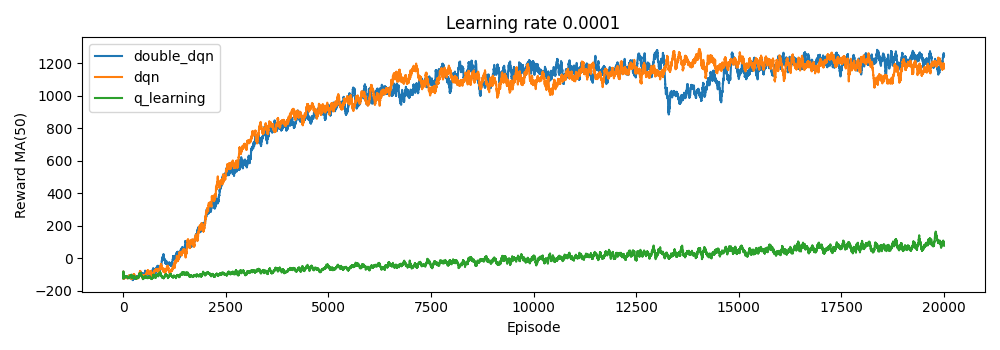
\includegraphics[width=0.85\textwidth]{image/reward_0001.png}
    \par\vspace{0.3cm}
    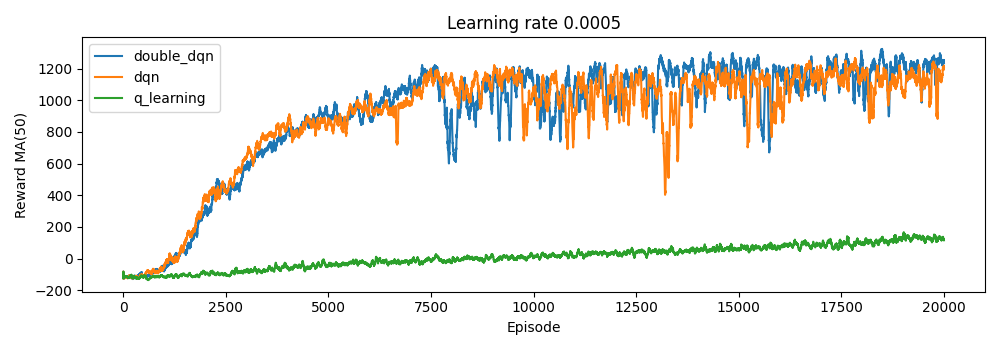
\includegraphics[width=0.85\textwidth]{image/reward_0005.png}
    \par\vspace{0.3cm}
    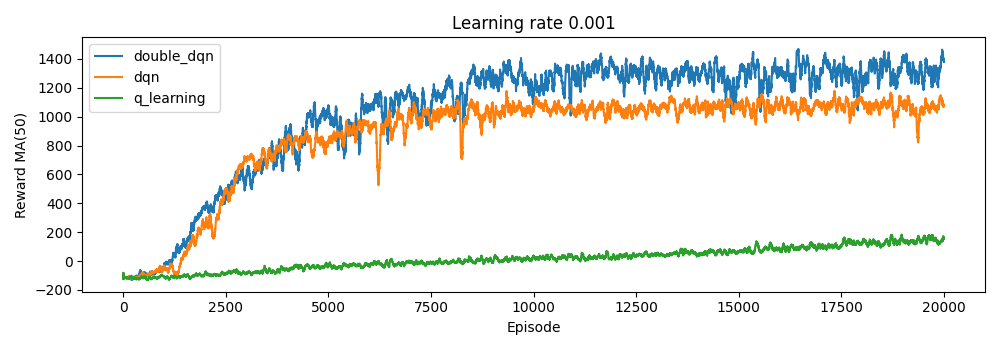
\includegraphics[width=0.85\textwidth]{image/reward_001.png}
    \caption{Reward trong quá trình training, được làm mượt bằng trung bình trượt 50 episode, với các mức learning rate lần lượt từ trên xuống dưới là $0{,}0001$, $0{,}0005$ và $0{,}001$.}
    \label{fig:reward-comparison}
\end{figure}

Reward tích lũy phản ánh tổng tác động của các sự kiện xảy ra trong một episode. Do nhiều thành phần reward có thể được cộng trong cùng một bước, chỉ số này cần được đọc cùng completion rate và win rate. \tabref{tab:reward-progress} trình bày reward trung bình từ các lần evaluation tại năm mốc training.

\begin{table}[H]
    \centering
    \renewcommand{\arraystretch}{1.2}
    \small
    \begin{tabular}{cccccc}
        \toprule
        \textbf{Cấu hình} & \makecell{\textbf{1.000}\\\textbf{episode}} & \makecell{\textbf{5.000}\\\textbf{episode}} & \makecell{\textbf{10.000}\\\textbf{episode}} & \makecell{\textbf{15.000}\\\textbf{episode}} & \makecell{\textbf{20.000}\\\textbf{episode}} \\
        \midrule
        Double DQN ($\mathrm{LR}=0{,}0001$) & $239{,}490$ & $946{,}191$ & $1195{,}874$ & $1159{,}812$ & $1247{,}154$ \\
        DQN ($\mathrm{LR}=0{,}0005$) & $302{,}023$ & $969{,}347$ & $982{,}988$ & $1257{,}292$ & $1254{,}443$ \\
        Q-Learning ($\mathrm{LR}=0{,}001$) & $-155{,}458$ & $-34{,}216$ & $16{,}860$ & $106{,}130$ & $165{,}472$ \\
        \bottomrule
    \end{tabular}
    \caption{Reward trung bình tại các mốc đánh giá.}
    \label{tab:reward-progress}
\end{table}

\figref{fig:reward-comparison} cho thấy reward training của DQN và Double DQN tăng nhanh trong giai đoạn đầu, sau đó dao động quanh mức cao. Tuy nhiên, reward tăng chưa đồng nghĩa với policy đã biết kết thúc màn chơi. Tại episode 5.000, Double DQN và DQN đạt reward evaluation lần lượt là $946{,}191$ và $969{,}347$, đồng thời đều thu thập hơn $95\%$ food. Dù vậy, hai cấu hình chỉ thắng lần lượt 1 và 0 trong 20 episode. Kết quả này cho thấy reward ở giai đoạn đó chủ yếu phản ánh khả năng thu thập phần lớn food và duy trì episode, còn khả năng hoàn thành vẫn chưa ổn định.

Đến episode 15.000, DQN đạt reward $1257{,}292$, completion rate $100\%$, win rate $100\%$ và chỉ cần trung bình $134{,}25$ bước. Sự thay đổi đồng thời của bốn chỉ số cho thấy policy không chỉ tạo reward cao hơn mà còn chuyển từ việc gần hoàn thành sang hoàn thành ổn định với ít bước hơn. Q-Learning cũng cải thiện reward từ $-155{,}458$ lên $165{,}472$, đi kèm completion rate tăng từ $8{,}39\%$ lên $46{,}29\%$. Tuy nhiên, win rate vẫn bằng $0\%$, nên mức reward tăng của Q-Learning chỉ phản ánh tiến bộ từng phần chứ chưa hình thành policy giải quyết hoàn chỉnh bài toán.

\subsubsection{Completion rate}

\begin{figure}[H]
    \centering
    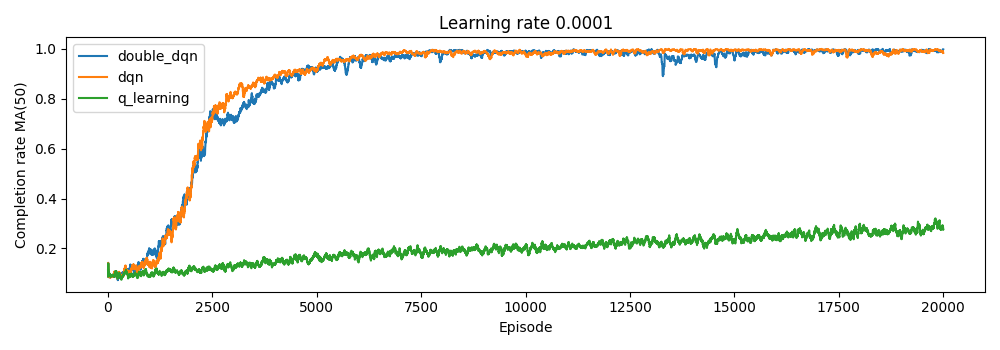
\includegraphics[width=0.85\textwidth]{image/completion_0001.png}
    \par\vspace{0.3cm}
    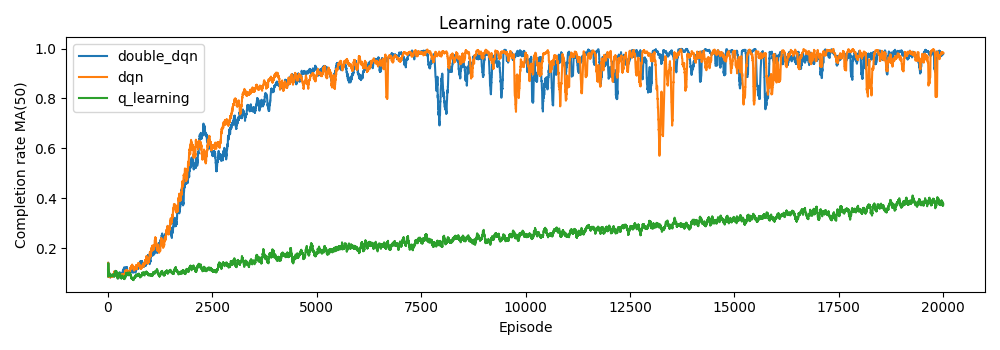
\includegraphics[width=0.85\textwidth]{image/completion_0005.png}
    \par\vspace{0.3cm}
    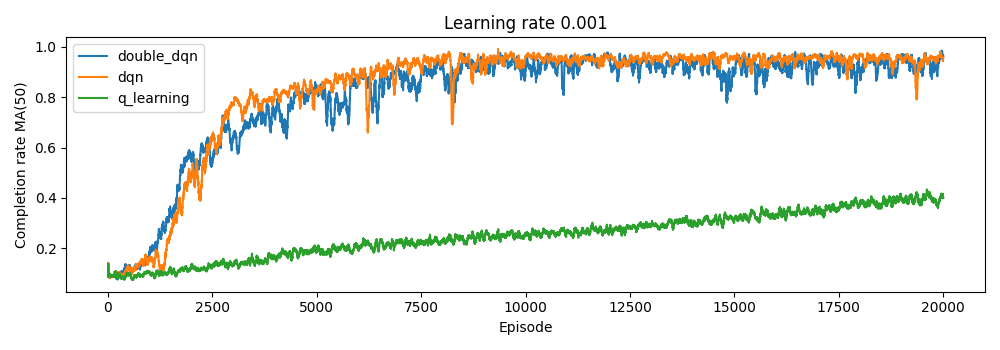
\includegraphics[width=0.85\textwidth]{image/completion_001.png}
    \caption{Completion rate trong quá trình training, được làm mượt bằng trung bình trượt 50 episode, với các mức learning rate lần lượt từ trên xuống dưới là $0{,}0001$, $0{,}0005$ và $0{,}001$.}
    \label{fig:completion-comparison}
\end{figure}

Completion rate biểu thị tỷ lệ food tác tử thu thập được trên tổng số 62 food của bản đồ. \tabref{tab:completion-progress} trình bày completion rate trung bình từ các lần evaluation tại năm mốc training.

\begin{table}[H]
    \centering
    \renewcommand{\arraystretch}{1.2}
    \small
    \begin{tabular}{cccccc}
        \toprule
        \textbf{Cấu hình} & \makecell{\textbf{1.000}\\\textbf{episode}} & \makecell{\textbf{5.000}\\\textbf{episode}} & \makecell{\textbf{10.000}\\\textbf{episode}} & \makecell{\textbf{15.000}\\\textbf{episode}} & \makecell{\textbf{20.000}\\\textbf{episode}} \\
        \midrule
        Double DQN ($\mathrm{LR}=0{,}0001$) & $49{,}11\%$ & $95{,}32\%$ & $99{,}03\%$ & $98{,}79\%$ & $99{,}76\%$ \\
        DQN ($\mathrm{LR}=0{,}0005$) & $58{,}71\%$ & $95{,}56\%$ & $91{,}21\%$ & $100{,}00\%$ & $99{,}84\%$ \\
        Q-Learning ($\mathrm{LR}=0{,}001$) & $8{,}39\%$ & $21{,}53\%$ & $27{,}74\%$ & $36{,}61\%$ & $46{,}29\%$ \\
        \bottomrule
    \end{tabular}
    \caption{Completion rate trung bình tại các mốc đánh giá.}
    \label{tab:completion-progress}
\end{table}

Completion rate giúp phân biệt hai mức độ học khác nhau: tìm được phần lớn food và thực sự hoàn thành episode. Tại episode 5.000, Double DQN đạt completion rate $95{,}32\%$ nhưng chỉ thắng 1/20 episode, còn DQN đạt $95{,}56\%$ nhưng không thắng episode nào. Như vậy, cả hai policy đã học được cách đi sâu vào mê cung và thu thập gần hết food, nhưng vẫn thường bị bắt trước khi lấy các food cuối cùng.

Khoảng cách giữa completion rate và win rate thu hẹp rõ rệt ở các checkpoint sau. DQN đạt đồng thời completion rate và win rate $100\%$ tại episode 15.000. Double DQN kết thúc training với completion rate $99{,}76\%$ và 19/20 episode chiến thắng. Ngược lại, Q-Learning tăng đều từ $8{,}39\%$ lên $46{,}29\%$ nhưng cả 20 episode evaluation cuối đều kết thúc do bị bắt. Q-Learning vì thế có học được hành vi thu thập food tốt hơn theo thời gian, song mức cải thiện chưa đủ để hoàn thành bản đồ.

\subsubsection{Win rate}

\begin{figure}[H]
    \centering
    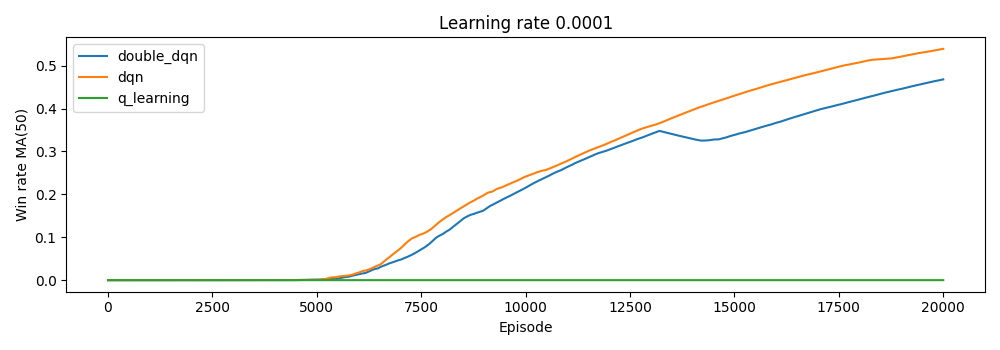
\includegraphics[width=0.85\textwidth]{image/win_rate_0001.png}
    \par\vspace{0.3cm}
    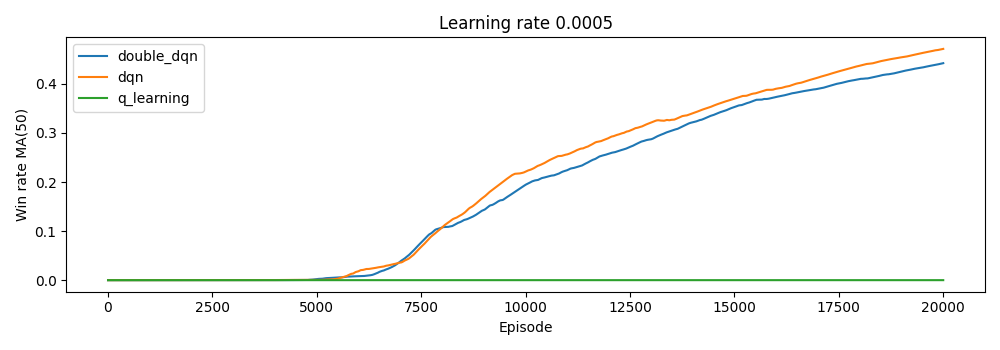
\includegraphics[width=0.85\textwidth]{image/win_rate_0005.png}
    \par\vspace{0.3cm}
    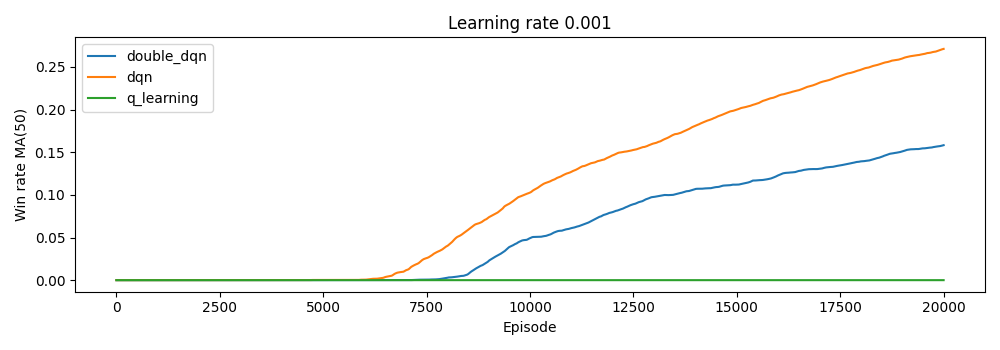
\includegraphics[width=0.85\textwidth]{image/win_rate_001.png}
    \caption{Tỷ lệ thắng tích lũy trong quá trình training, được làm mượt bằng trung bình trượt 50 episode, với các mức learning rate lần lượt từ trên xuống dưới là $0{,}0001$, $0{,}0005$ và $0{,}001$.}
    \label{fig:winrate-comparison}
\end{figure}

Win rate trên đồ thị là tỷ lệ thắng tích lũy từ đầu quá trình training. Trong khi đó, \tabref{tab:winrate-progress} sử dụng win rate của 20 episode evaluation độc lập tại từng checkpoint. Ở cả hai trường hợp, một episode được tính là thắng khi tác tử thu thập đủ 62 food.

\begin{table}[H]
    \centering
    \renewcommand{\arraystretch}{1.2}
    \small
    \begin{tabular}{cccccc}
        \toprule
        \textbf{Cấu hình} & \makecell{\textbf{10.000}\\\textbf{episode}} & \makecell{\textbf{11.000}\\\textbf{episode}} & \makecell{\textbf{12.000}\\\textbf{episode}} & \makecell{\textbf{15.000}\\\textbf{episode}} & \makecell{\textbf{20.000}\\\textbf{episode}} \\
        \midrule
        Double DQN ($\mathrm{LR}=0{,}0001$) & $80\%$ & $95\%$ & $85\%$ & $80\%$ & $95\%$ \\
        DQN ($\mathrm{LR}=0{,}0005$) & $45\%$ & $0\%$ & $100\%$ & $100\%$ & $95\%$ \\
        Q-Learning ($\mathrm{LR}=0{,}001$) & $0\%$ & $0\%$ & $0\%$ & $0\%$ & $0\%$ \\
        \bottomrule
    \end{tabular}
    \caption{Win rate tại các mốc đánh giá.}
    \label{tab:winrate-progress}
\end{table}

Win rate cho thấy thời điểm policy chuyển từ gần hoàn thành sang hoàn thành thực sự. DQN có win rate $45\%$ tại episode 10.000, thấp hơn mức $80\%$ của Double DQN. Sau đó, DQN biến động mạnh và đạt $100\%$ tại episode 12.000, đồng thời duy trì mức này ở episode 15.000.

Dao động lớn nhất xuất hiện ở DQN tại episode 11.000. Reward giảm từ $982{,}988$ xuống $138{,}031$, completion rate giảm từ $91{,}21\%$ xuống $38{,}31\%$ và cả 20 episode đều kết thúc do bị bắt. Ngay tại episode 12.000, policy lại thắng 20/20 episode với completion rate $100\%$. Sự suy giảm đồng thời trên nhiều metric cho thấy đây là một checkpoint có hiệu năng thấp, không chỉ là biến động riêng của win rate. Dù vậy, một training seed chưa đủ để quy nguyên nhân cho catastrophic forgetting. Double DQN cũng dao động từ $95\%$ ở episode 11.000 xuống $80\%$ ở episode 15.000, nhưng không xuất hiện mức sụt về $0\%$ như DQN.

\subsubsection{Steps}

\begin{figure}[H]
    \centering
    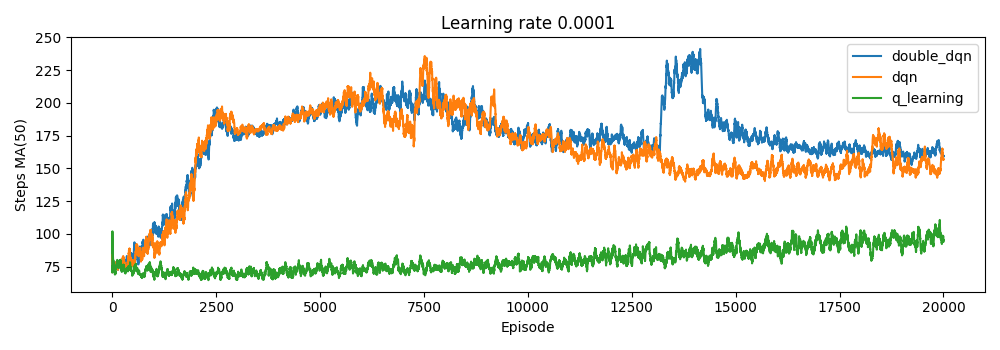
\includegraphics[width=0.85\textwidth]{image/steps_0001.png}
    \par\vspace{0.3cm}
    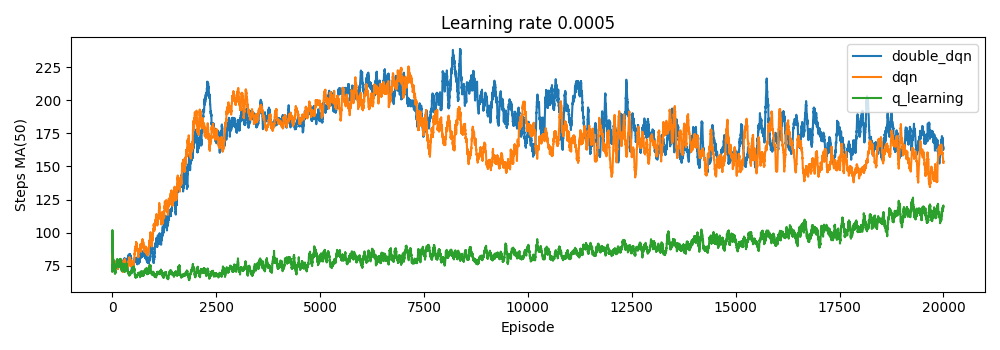
\includegraphics[width=0.85\textwidth]{image/steps_0005.png}
    \par\vspace{0.3cm}
    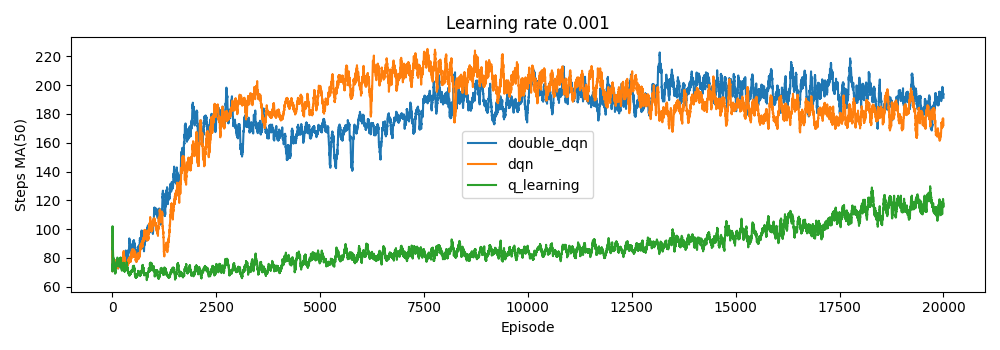
\includegraphics[width=0.85\textwidth]{image/steps_001.png}
    \caption{Số bước trong quá trình training, được làm mượt bằng trung bình trượt 50 episode, với các mức learning rate lần lượt từ trên xuống dưới là $0{,}0001$, $0{,}0005$ và $0{,}001$.}
    \label{fig:steps-comparison}
\end{figure}

Số bước trung bình phản ánh độ dài của episode trước khi tác tử thắng, mất mạng cuối cùng hoặc đạt giới hạn bước. Vì episode thất bại sớm cũng có thể có ít bước, chỉ số này phải được đọc cùng win rate và completion rate. \tabref{tab:steps-progress} trình bày số bước trung bình từ các lần evaluation tại năm mốc training.

\begin{table}[H]
    \centering
    \renewcommand{\arraystretch}{1.2}
    \small
    \begin{tabular}{cccccc}
        \toprule
        \textbf{Cấu hình} & \makecell{\textbf{1.000}\\\textbf{episode}} & \makecell{\textbf{5.000}\\\textbf{episode}} & \makecell{\textbf{10.000}\\\textbf{episode}} & \makecell{\textbf{15.000}\\\textbf{episode}} & \makecell{\textbf{20.000}\\\textbf{episode}} \\
        \midrule
        Double DQN ($\mathrm{LR}=0{,}0001$) & $219{,}00$ & $235{,}60$ & $163{,}25$ & $176{,}35$ & $148{,}30$ \\
        DQN ($\mathrm{LR}=0{,}0005$) & $210{,}90$ & $229{,}95$ & $177{,}85$ & $134{,}25$ & $138{,}90$ \\
        Q-Learning ($\mathrm{LR}=0{,}001$) & $66{,}00$ & $85{,}20$ & $89{,}05$ & $99{,}60$ & $134{,}40$ \\
        \bottomrule
    \end{tabular}
    \caption{Số bước trung bình tại các mốc đánh giá.}
    \label{tab:steps-progress}
\end{table}

Số bước chỉ có ý nghĩa khi được đối chiếu với kết quả kết thúc episode. Tại episode 5.000, DQN và Double DQN cần trung bình khoảng 230 bước, đạt completion rate trên $95\%$ nhưng gần như không thắng. Các episode dài ở giai đoạn này cho thấy tác tử đã tồn tại đủ lâu để thu thập phần lớn food, nhưng chưa hoàn thành được phần cuối của bản đồ. Đến episode 15.000, DQN thắng 20/20 episode và số bước giảm còn $134{,}25$. Việc số bước giảm đồng thời với win rate tăng cho thấy policy đã hoàn thành episode hiệu quả hơn, thay vì kết thúc sớm do bị bắt.

Tại lần evaluation cuối, DQN và Double DQN cùng thắng 19/20 episode, với số bước trung bình lần lượt là $138{,}90$ và $148{,}30$. DQN sử dụng ít bước hơn trong cùng điều kiện hoàn thành gần tương đương, nhưng dữ liệu chưa đủ để khẳng định đây là đường đi ngắn nhất. Đối với Q-Learning, số bước tăng từ $66{,}00$ lên $134{,}40$ cùng với completion rate tăng từ $8{,}39\%$ lên $46{,}29\%$. Vì tất cả episode cuối vẫn kết thúc do bị bắt, xu hướng này phản ánh khả năng tồn tại và thu thập food được cải thiện, không phải hiệu quả hoàn thành.

\subsubsection{Loss}

\begin{figure}[H]
    \centering
    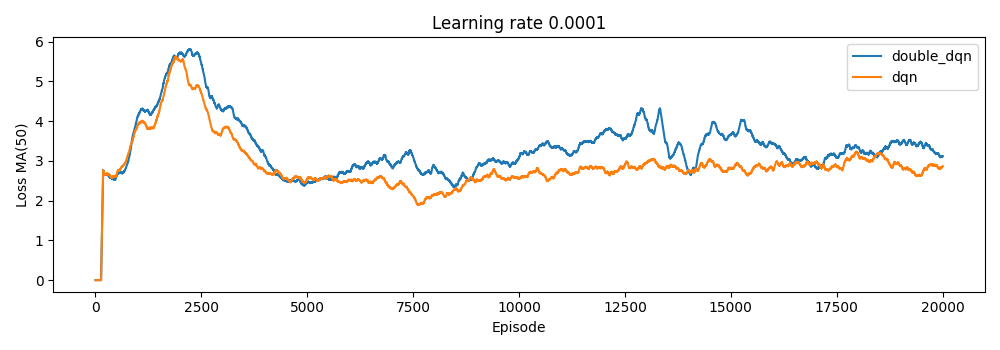
\includegraphics[width=0.85\textwidth]{image/loss_0001.png}
    \par\vspace{0.3cm}
    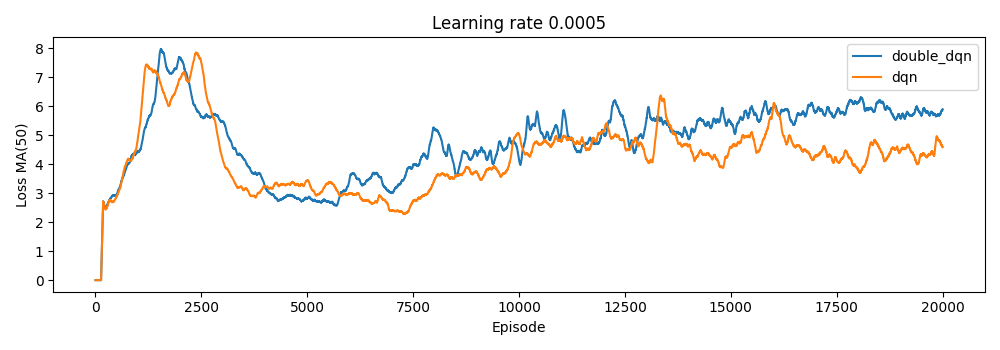
\includegraphics[width=0.85\textwidth]{image/loss_0005.png}
    \par\vspace{0.3cm}
    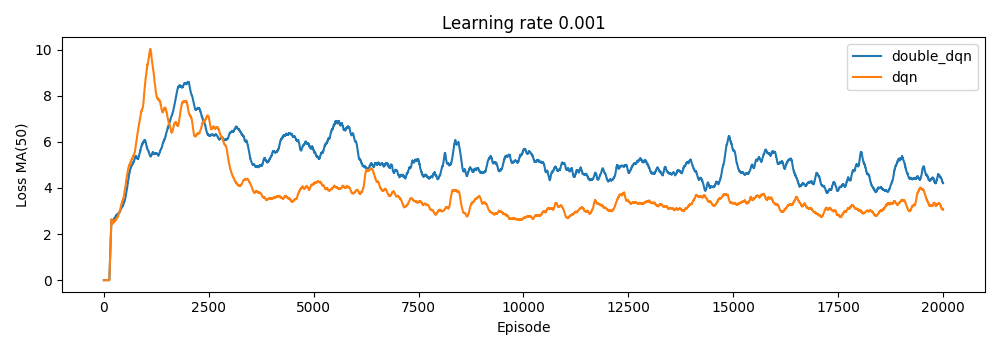
\includegraphics[width=0.85\textwidth]{image/loss_001.png}
    \caption{Smooth L1 Loss trong quá trình training, được làm mượt bằng trung bình trượt 50 episode, với các mức learning rate lần lượt từ trên xuống dưới là $0{,}0001$, $0{,}0005$ và $0{,}001$.}
    \label{fig:loss-comparison}
\end{figure}

Smooth L1 Loss chỉ áp dụng cho DQN và Double DQN. Chỉ số này là trung bình loss của các lần cập nhật mạng trong một episode training. \tabref{tab:loss-progress} tổng hợp giá trị tại một số mốc của hai cấu hình có win rate cuối cao nhất.

\begin{table}[H]
    \centering
    \renewcommand{\arraystretch}{1.2}
    \small
    \begin{tabular}{ccccc}
        \toprule
        \textbf{Cấu hình} & \makecell{\textbf{5.000}\\\textbf{episode}} & \makecell{\textbf{10.000}\\\textbf{episode}} & \makecell{\textbf{15.000}\\\textbf{episode}} & \makecell{\textbf{20.000}\\\textbf{episode}} \\
        \midrule
        DQN ($\mathrm{LR}=0{,}0005$) & $3{,}42$ & $4{,}74$ & $4{,}60$ & $4{,}78$ \\
        Double DQN ($\mathrm{LR}=0{,}0001$) & $2{,}43$ & $3{,}28$ & $3{,}67$ & $2{,}86$ \\
        \bottomrule
    \end{tabular}
    \caption{Loss trung bình trong episode tại các mốc training.}
    \label{tab:loss-progress}
\end{table}

Trước khi replay buffer tích lũy đủ 10.000 environment step, loss bằng $0$ vì online network chưa được cập nhật. Khi quá trình tối ưu bắt đầu, loss tăng nhanh rồi chuyển sang trạng thái dao động. Loss không giảm đều về $0$ do target thay đổi theo chính policy đang học và phân phối mẫu trong replay buffer cũng liên tục biến đổi.

DQN với $\mathrm{LR}=0{,}0005$ có loss $4{,}60$ tại episode 15.000 và $4{,}78$ tại episode 20.000, dù win rate tương ứng là $100\%$ và $95\%$. Điều này cho thấy loss không cần đạt giá trị nhỏ nhất để policy có hiệu năng cao. Double DQN với $\mathrm{LR}=0{,}0001$ có loss thấp hơn tại các mốc được thống kê, nhưng hai cấu hình sử dụng learning rate khác nhau nên không thể quy toàn bộ chênh lệch cho cơ chế Double DQN. Loss vì thế chỉ được dùng để theo dõi quá trình cập nhật mạng, còn chất lượng policy phải được đánh giá bằng reward, completion rate và win rate.

\subsection{Ảnh hưởng của learning rate}

Learning rate ($\alpha$) ảnh hưởng khác nhau đến từng thuật toán. \tabref{tab:lr-trend} sắp xếp kết quả theo thứ tự $\mathrm{LR}=0{,}0001 \rightarrow 0{,}0005 \rightarrow 0{,}001$ để thể hiện trực tiếp xu hướng của từng chỉ số.

\begin{table}[H]
    \centering
    \renewcommand{\arraystretch}{1.2}
    \setlength{\tabcolsep}{4pt}
    \footnotesize
    \begin{tabular}{lccc}
        \toprule
        \textbf{Thuật toán} & \textbf{Số thắng/20} & \textbf{Completion rate (\%)} & \textbf{Steps} \\
        \midrule
        Q-Learning & $0 \rightarrow 0 \rightarrow 0$ & $26{,}29 \rightarrow 42{,}66 \rightarrow 46{,}29$ & $99{,}25 \rightarrow 124{,}05 \rightarrow 134{,}40$ \\
        DQN & $15 \rightarrow 19 \rightarrow 15$ & $98{,}55 \rightarrow 99{,}84 \rightarrow 98{,}71$ & $157{,}85 \rightarrow 138{,}90 \rightarrow 161{,}85$ \\
        Double DQN & $19 \rightarrow 17 \rightarrow 13$ & $99{,}76 \rightarrow 99{,}27 \rightarrow 99{,}27$ & $148{,}30 \rightarrow 153{,}60 \rightarrow 211{,}65$ \\
        \bottomrule
    \end{tabular}
    \caption{Xu hướng kết quả khi learning rate tăng từ $0{,}0001$ lên $0{,}001$ \cite{DRLPacmanGitHub}.}
    \label{tab:lr-trend}
\end{table}

\noindent\textbf{Q-Learning.} Trong ba cấu hình đã chạy, learning rate tăng đi kèm với reward, completion rate và số bước trung bình cùng tăng. $\mathrm{LR}=0{,}001$ đạt reward $165{,}472$ và completion rate $46{,}29\%$, cao hơn hai mức còn lại, nhưng cả 20 episode evaluation vẫn kết thúc do bị bắt. Như vậy, learning rate lớn hơn giúp policy đi xa hơn và thu thập nhiều food hơn trong miền đã khảo sát, song chưa làm thay đổi kết quả cuối cùng là win rate $0\%$. Do learning rate lớn nhất mới chỉ bằng $0{,}001$, thí nghiệm chưa xác định được mức phù hợp nhất cho cập nhật Q-table.

\noindent\textbf{DQN.} Hai mức còn lại là $\mathrm{LR}=0{,}0001$ và $\mathrm{LR}=0{,}001$ đều thắng 15/20 episode, trong khi $\mathrm{LR}=0{,}0005$ thắng 19/20 episode. Cấu hình này cũng có completion rate cao nhất là $99{,}84\%$ và số bước thấp nhất là $138{,}90$. Cả ba chỉ số đều cho thấy $\mathrm{LR}=0{,}0005$ là cấu hình cân bằng nhất của DQN trong miền đã khảo sát. Tuy nhiên, ba điểm dữ liệu và một training seed chưa đủ để kết luận quan hệ giữa learning rate và hiệu năng có dạng cụ thể.

\noindent\textbf{Double DQN.} Khi learning rate tăng, số episode thắng giảm lần lượt từ 19 xuống 17 và 13, trong khi số episode bị bắt tăng từ 1 lên 3 và 7. Completion rate của cả ba cấu hình vẫn trên $99\%$, cho thấy các episode thất bại thường kết thúc khi tác tử đã thu thập gần hết food. Đồng thời, reward tăng từ $1247{,}154$ lên $1553{,}422$ và số bước tăng từ $148{,}30$ lên $211{,}65$. Vì log không tách reward theo sự kiện, chưa thể xác định nguồn reward tăng thêm. Tuy nhiên, kết quả đủ cho thấy $\mathrm{LR}=0{,}001$ tạo ra policy có reward cao nhưng mất nhiều bước hơn và bị bắt thường xuyên hơn. Xét mục tiêu hoàn thành màn chơi, $\mathrm{LR}=0{,}0001$ là cấu hình phù hợp nhất của Double DQN trong ba mức đã thử.

\subsection{Tổng hợp kết quả thực nghiệm}

Tại episode 20.000, \tabref{tab:representative-comparison} đối chiếu cấu hình có win rate cao nhất của từng thuật toán. Cột kết quả lần lượt ghi số episode thắng, bị bắt và timeout trong 20 episode evaluation.

\begin{table}[H]
    \centering
    \renewcommand{\arraystretch}{1.2}
    \setlength{\tabcolsep}{5pt}
    \footnotesize
    \begin{tabular}{lcccc}
        \toprule
        \textbf{Cấu hình} & \makecell{\textbf{Thắng/Bị bắt}\\\textbf{/Timeout}} & \textbf{Reward} & \makecell{\textbf{Completion}\\\textbf{rate}} & \textbf{Steps} \\
        \midrule
        Q-Learning ($\mathrm{LR}=0{,}001$) & $0/20/0$ & $165{,}472$ & $46{,}29\%$ & $134{,}40$ \\
        DQN ($\mathrm{LR}=0{,}0005$) & $19/1/0$ & $1254{,}443$ & $99{,}84\%$ & $138{,}90$ \\
        Double DQN ($\mathrm{LR}=0{,}0001$) & $19/1/0$ & $1247{,}154$ & $99{,}76\%$ & $148{,}30$ \\
        \bottomrule
    \end{tabular}
    \caption{Đối chiếu ba cấu hình đại diện tại episode 20.000 \cite{DRLPacmanGitHub}.}
    \label{tab:representative-comparison}
\end{table}

Q-Learning không thắng episode nào và cả 20 episode đều kết thúc do bị bắt. Completion rate $46{,}29\%$ cho thấy tác tử đã học được cách thu thập một phần food, nhưng chưa học được policy hoàn thành bản đồ.

DQN và Double DQN có cùng số episode thắng và cùng số lần bị bắt. DQN có completion rate cao hơn $0{,}08$ điểm phần trăm và sử dụng ít hơn trung bình $9{,}40$ bước. Chênh lệch này ủng hộ việc chọn DQN $\mathrm{LR}=0{,}0005$ khi ưu tiên số bước, nhưng một training seed chưa đủ để khẳng định DQN tốt hơn Double DQN về tổng quát.

Reward cũng không thể được dùng làm tiêu chí duy nhất. Double DQN với $\mathrm{LR}=0{,}001$ đạt reward cao nhất là $1553{,}422$, nhưng chỉ thắng 13/20 episode, bị bắt 7 lần và cần trung bình $211{,}65$ bước. Vì vậy, DQN $\mathrm{LR}=0{,}0005$ và Double DQN $\mathrm{LR}=0{,}0001$ là hai cấu hình cân bằng nhất khi xét đồng thời win rate, completion rate và số bước.

\subsection{Hạn chế của thực nghiệm}

Mỗi cấu hình chỉ được training một lần với seed 42. Vì chưa có các lần chạy độc lập, báo cáo chưa xác định được độ biến động giữa các seed, độ lệch chuẩn hoặc khoảng tin cậy. Những chênh lệch nhỏ giữa các cấu hình vì thế cần được diễn giải thận trọng.

Mỗi lần evaluation gồm 20 episode với seed 10042 nên win rate thay đổi theo bước $5\%$. Seed cố định tạo điều kiện so sánh nhất quán, nhưng chưa phản ánh hiệu năng trên nhiều chuỗi ngẫu nhiên. Log cũng chỉ lưu reward tổng, chưa tách đóng góp của các sự kiện như ăn ghost, bonus fruit hoặc va tường.

Q-Learning dùng tuple state 17 giá trị, còn DQN và Double DQN dùng vector 92 chiều với nhiều thông tin bổ sung. Chênh lệch kết quả do đó chịu ảnh hưởng đồng thời của thuật toán và cách biểu diễn state. Thiết kế hiện tại chưa tách riêng hai yếu tố này.

Ba learning rate được dùng chung cho cả ba thuật toán, dù chúng tác động lên Q-table và optimizer Adam theo cách khác nhau. Miền khảo sát chưa chắc chứa cấu hình tốt nhất cho từng phương pháp. Kết quả chỉ cho phép so sánh ba mức đã chọn.

Thực nghiệm mới được thực hiện trên bản đồ \texttt{medium}, với ba ma, ba mạng sống và một thiết kế reward cố định. Khả năng khái quát sang điều kiện khác cần được kiểm chứng bằng thí nghiệm bổ sung.

\subsection{Hướng dẫn chạy demo}

Demo cho phép lựa chọn một trong chín final model đã huấn luyện của Q-Learning, DQN và Double DQN. Trong quá trình chạy, tác tử chỉ sử dụng policy đã lưu để lựa chọn action. Q-table và tham số mạng không được cập nhật. Các lệnh dưới đây được thực hiện trong PowerShell tại thư mục gốc của repository \cite{DRLPacmanGitHub}.

\begin{enumerate}
    \item \textbf{Chuẩn bị môi trường.} Bước này chỉ cần thực hiện trong lần chạy đầu tiên.

    {\small
    \begin{verbatim}
conda create -n pacman python=3.10 -y
conda activate pacman
pip install -r requirements.txt
    \end{verbatim}
    }

    \item \textbf{Mở danh sách lựa chọn model.} Chạy lệnh sau để chương trình quét thư mục \texttt{models/final} và hiển thị các model hiện có.

    {\small
    \begin{verbatim}
python -m src.training.watch_finals
    \end{verbatim}
    }

    Mỗi dòng trong danh sách gồm số thứ tự, thuật toán, learning rate và đường dẫn tới final model. Người dùng nhập số tương ứng rồi nhấn \texttt{Enter} để chạy model. Chẳng hạn, nhập \texttt{5} để chọn DQN với $\mathrm{LR}=0{,}0005$, là cấu hình DQN có kết quả cuối tốt nhất trong thực nghiệm. Lựa chọn \texttt{a} dùng để chạy lần lượt toàn bộ model. Giao diện lựa chọn được minh họa trong \figref{fig:demo-model-selection}.

    \begin{figure}[H]
        \centering
        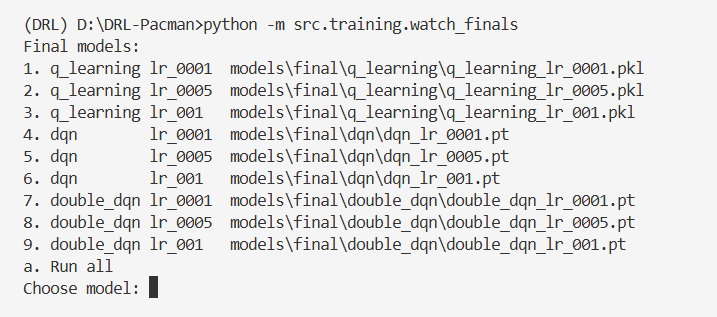
\includegraphics[width=0.82\textwidth]{image/choose_model.png}
        \caption{Danh sách lựa chọn final model khi chạy demo.}
        \label{fig:demo-model-selection}
    \end{figure}

    \item \textbf{Quan sát tác tử.} Sau khi model được chọn, cửa sổ Mini Pacman mở và policy tự động điều khiển Pacman. Phần trên của giao diện hiển thị episode hiện tại, số bước, action vừa chọn và sự kiện trong môi trường. Mặc định, chương trình chạy ba episode với độ trễ 500 ms giữa hai bước.

    Khi Pacman thu thập đủ 62 food, episode kết thúc với thông báo \textit{You Win}. Nếu Pacman mất mạng cuối cùng hoặc chạm giới hạn số bước, giao diện hiển thị \textit{You Lose}. Hai trạng thái kết thúc được thể hiện trong \figref{fig:demo-results}.

    \begin{figure}[H]
        \centering
        \begin{subfigure}[t]{0.39\textwidth}
            \centering
            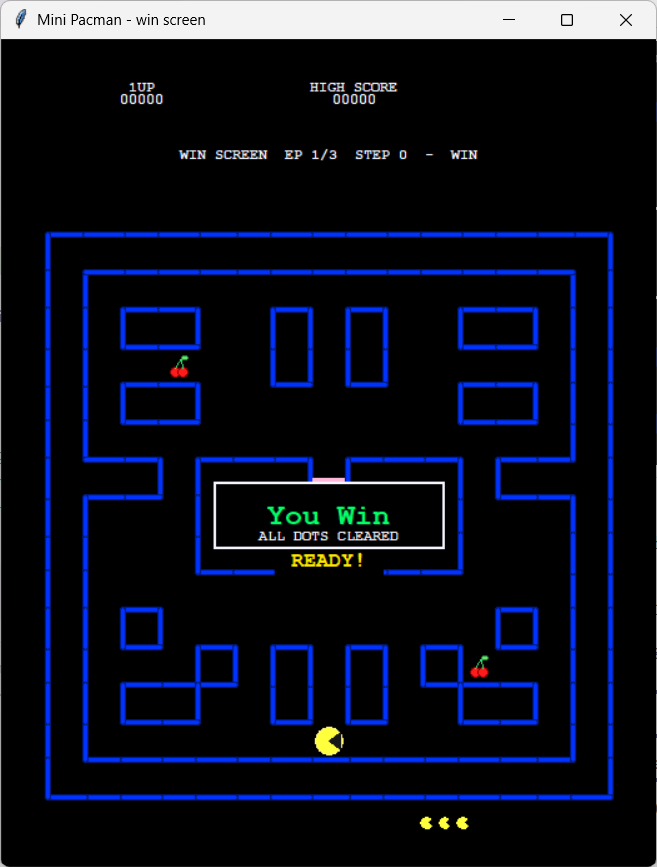
\includegraphics[width=\textwidth]{image/pacman_win.png}
            \caption{Pacman hoàn thành bản đồ.}
            \label{fig:demo-win}
        \end{subfigure}%
        \hspace{0.025\textwidth}%
        \begin{subfigure}[t]{0.39\textwidth}
            \centering
            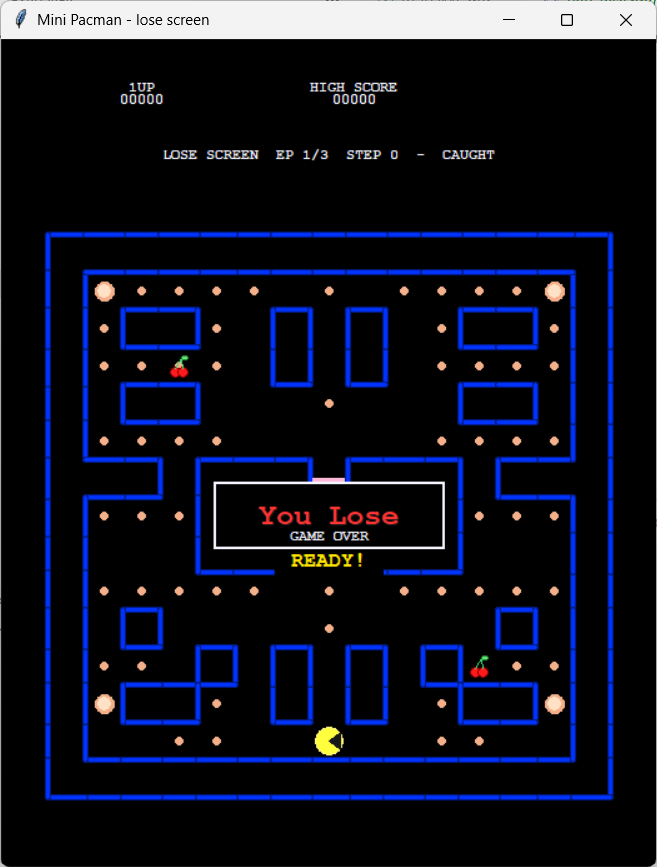
\includegraphics[width=\textwidth]{image/pacman_lose.png}
            \caption{Pacman kết thúc episode do bị bắt.}
            \label{fig:demo-lose}
        \end{subfigure}
        \caption{Hai trạng thái kết thúc có thể quan sát trong giao diện demo.}
        \label{fig:demo-results}
    \end{figure}

    \item \textbf{Điều chỉnh hiển thị.} Số episode và tốc độ hiển thị có thể được thay đổi bằng các tham số sau.

    {\small
    \begin{verbatim}
python -m src.training.watch_finals --episodes 5 --delay-ms 150
    \end{verbatim}
    }

    Trong lệnh trên, \texttt{--episodes 5} đặt số episode chạy cho model được chọn, còn \texttt{--delay-ms 150} rút ngắn thời gian chờ giữa hai bước xuống 150 ms. Sau khi nhập lệnh, người dùng vẫn chọn model từ danh sách như ở bước 2.
\end{enumerate}

Người dùng có thể đóng cửa sổ Mini Pacman tại bất kỳ thời điểm nào để kết thúc demo hiện tại.
